\documentclass[10pt]{article}
\usepackage{icmlko}

\icmlmeta{IP 파운데이션 월드모델}{280}{청력 곡선}{정식화 일곱 x 도메인 다섯 --- 나무의 문턱이 예측한 40행에 정확히 있고, 도메인별 배합은 그보다 여섯 배 높다}

\begin{document}

\twocolumn[
\icmlheader

\begin{abstract}
노트 279가 두 점(팝업 16행 · 웹툰 2,106행)으로 ``청력''을 세웠다. 사이를
메웠다 --- 아이돌 54 · 도서 80 · 게임 259. \textbf{정식화마다 곡선 모양이
다르고 넷으로 갈린다.} ① \textbf{문턱 없음}(F6 · F9 순수 풀링) --- 16행에서
이미 $+$0.53 · $+$0.63 이고 크기와 거의 무관하다. ② \textbf{40행 계단}(F8 ·
F18 나무) --- 16행 \textbf{0.0000}, 54행 \textbf{$+$0.6623 · $+$0.5677}.
노트 276이 \texttt{min\_samples\_leaf}$=$20 에서 예측한 자리가
$2{\times}20{=}40$ 인데 \textbf{계단이 정확히 거기 있다.} ③ \textbf{완만한
경사}(F21 · F23) --- 0.088 $\to$ 0.246 $\to$ 0.311 $\to$ 0.314 $\to$ 0.596,
문턱이 아니라 비탈이다. ④ \textbf{80$\sim$259 계단}(F10 도메인별 배합) ---
16 · 54 · 80행에서 \textbf{전부 정확히 0} 이다가 259행에서 $+$0.4034,
2,106행에서 \textbf{$+$0.7354(전체 최고)}. \textbf{제일 잘 듣는 정식화가
제일 늦게 듣기 시작한다.} 챔피언 F18의 문턱은 40행이고, 판정치는 이 수를
한 번도 보고한 적이 없다. \textbf{그리고 이 곡선은 다음 도메인을 고르는
자리에서 바로 쓰인다} --- 2호 도메인 아이돌의 첫 뱅크가 $n{\approx}250$
이라 F10만 빼면 전부 문턱 위다. \emph{바로잡음}: 노트 276$\sim$279가 누출
열의 팝업 관측행을 ``14''로 적었는데 \textbf{16}이 맞다(14는 진짜
\texttt{pop\_*} 축의 덮음). 둘 다 20 아래라 결론은 안 바뀐다.
\end{abstract}
]

\section{두 점을 다섯 점으로}

노트 279가 웹툰과 팝업 두 점으로 ``눈먼 정식화는 없고 청력 차이만 있다''를
세웠다. 두 점으로는 \textbf{선}밖에 못 그린다 --- 문턱인지 비탈인지 모른다.

세 도메인을 채웠다. 눈금은 그대로다 --- 도메인마다 \textbf{라벨 순위를
그대로} 전용 열로 주고 그 도메인 $\rho$ 가 얼마나 오르는지 본다.
\textbf{진단 전용이고 채택은 없다.}

\begin{figure*}[t]
\centering
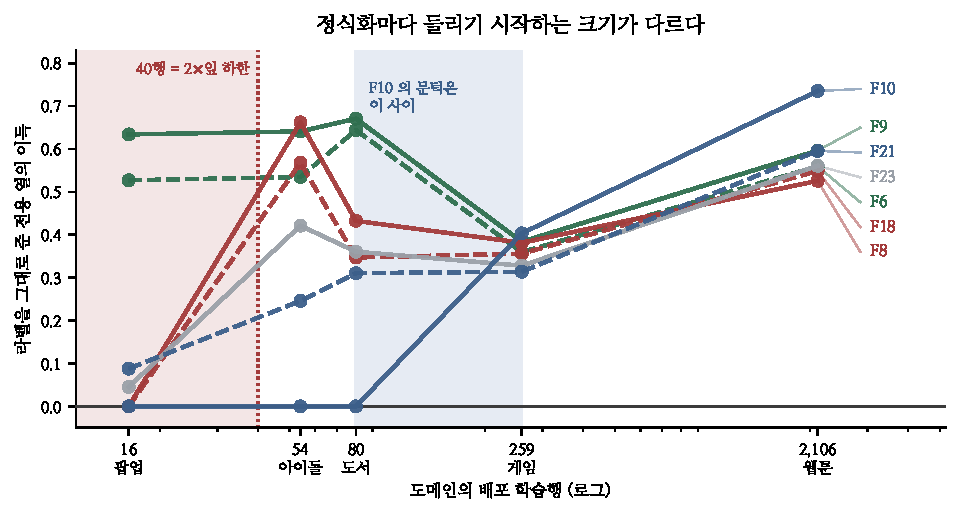
\includegraphics[width=\textwidth]{figs/curve.pdf}
\caption{정식화 일곱의 청력 곡선. 붉은 띠가 40행($2{\times}$잎 하한) 아래,
푸른 띠가 F10의 문턱이 있는 구간. 초록 순수 풀링 · 붉은 나무 · 파랑
도메인별 배합 · 회색 반반 섞음.}
\end{figure*}

\begin{center}\small
\begin{tabular}{lrrrrr}
\hline
& 16 & 54 & 80 & 259 & 2,106 \\
& 팝업 & 아이돌 & 도서 & 게임 & 웹툰 \\
\hline
F9 & .634 & .641 & .671 & .384 & .596 \\
F6 & .527 & .535 & .644 & .360 & .560 \\
\hline
F8 & \textbf{.000} & .662 & .433 & .382 & .526 \\
F18 & \textbf{.000} & .568 & .347 & .356 & .549 \\
\hline
F23 & .045 & .421 & .361 & .328 & .561 \\
F21 & .088 & .246 & .311 & .314 & .596 \\
\hline
F10 & \textbf{.000} & \textbf{.000} & \textbf{.000} & .403 & \textbf{.735} \\
\hline
\end{tabular}
\end{center}

\section{네 가지 모양}

\paragraph{① 문턱 없음 --- F6 · F9(순수 풀링)} 16행에서 이미 $+$0.527 ·
$+$0.634 이고 2,106행에서 $+$0.560 · $+$0.596 이다. \textbf{크기를 130배
늘려도 안 달라진다.} 전 도메인을 한 표로 놓고 계수를 푸니 16행짜리 열도 제
계수를 받는다.

\paragraph{② 40행 계단 --- F8 · F18(나무)} \textbf{이 노트에서 제일 값진
수다.} 노트 276이 범인을 \texttt{min\_samples\_leaf}$=$20 으로 지목하면서
``양쪽 잎을 채우려면 40행''이라고 적었다. 그건 \emph{예측}이었고 점이 둘밖에
없었다. 이제 셋이다 --- 16행 \textbf{0.0000}, 54행 $+$0.662 · $+$0.568.
\textbf{계단이 예측한 자리에 있다.}

\paragraph{③ 완만한 경사 --- F21 · F23} F21이 .088 $\to$ .246 $\to$ .311
$\to$ .314 $\to$ .596 이다. \textbf{문턱이 아니라 비탈이다} --- 도메인별
배합비가 연속량이라 제 이력이 두꺼워질수록 조금씩 제 쪽으로 옮겨 간다.
F23은 정의상 F21과 F18의 반반이라 둘 사이에 눕는다(16행에서 .045 $\approx$
$(.088{+}0)/2$, 54행에서 .421 $\approx$ $(.246{+}.568)/2{=}.407$).
\textbf{반반 산수가 다섯 점 중 둘에서 다시 닫힌다.}

\paragraph{④ 80$\sim$259 계단 --- F10} 16 · 54 · 80행에서 \emph{전부 정확히}
0 이다가 259행에서 $+$0.403, 2,106행에서 $+$0.735 다. \textbf{문턱이 나무보다
여섯 배 이상 높다.} 그런데 문턱을 넘고 나면 \textbf{일곱 중 제일 잘 듣는다.}
같은 기전이 양쪽을 만든다 --- 배합이 제 이력 쪽으로 완전히 넘어가면 제
전용 열이 최대로 일하고, 안 넘어가면 통째로 버려진다. \textbf{제일 잘 듣는
것이 제일 늦게 듣기 시작한다.}

\paragraph{게임 259가 전체적으로 낮다} 일곱 다 0.31$\sim$0.40 으로 눌려
있다(다른 크기에서는 0.35$\sim$0.74). 게임은 정상 $\rho$ 가 이미 0.59$\sim$
0.63 으로 제일 높아서 \textbf{올릴 자리가 좁다} --- 누출 뒤 값이 0.93$\sim$
0.99 로 다른 도메인과 같으니 천장 효과다. 청력 자체의 문제가 아니다.

\section{이 표를 어디에 쓰나}

\paragraph{챔피언의 문턱은 40행이다} 지금 챔피언은 F18이고 그 청력 문턱이
\textbf{40행}이다. 판정치는 이 수를 한 번도 낸 적이 없다 --- 노트 279가
잰 대로 판 $\rho$ 는 웹툰 27.3\% · 애니 23.6\% 가 절반이라 정식화들이
서로 같아지는 자리에서만 잰다.

\paragraph{다음 도메인을 고르는 자리에서 바로 쓰인다} 2호 도메인 아이돌의
첫 뱅크가 $n{\approx}250$ 이고 그중 학습에 들어갈 몫은 더 작다. 이 표로
읽으면 이렇다.

\begin{center}\small
\begin{tabular}{lll}
\hline
학습행 & 쓸 수 있는 정식화 & 못 쓰는 것 \\
\hline
$<$40 & F6 · F9 (· F21 · F23 약하게) & F8 · F18 · F10 \\
40$\sim$250 & 위 $+$ F8 · F18 & F10 \\
$>$250 & 일곱 다 & --- \\
\hline
\end{tabular}
\end{center}

\textbf{새 도메인의 전용 축을 쓸 계획이 있으면 학습행이 40을 넘는지부터
본다.} 그 아래면 챔피언이 그 축을 통째로 무시하고, 그 사실은 판에 한 자리도
안 나타난다.

\paragraph{그래도 눈금은 안 바꾼다} 노트 268의 규약이 산다. 그리고 이
곡선은 \textbf{라벨을 통째로 준 진단용 열}로 그린 것이라 상한이지 실측이
아니다 --- 노트 277이 확인한 대로 진짜 팝업 축 넷은 능형에서도 $-$0.0070
이다. \textbf{청력이 있다고 들을 말이 있는 것은 아니다.}

\paragraph{바로잡음} 노트 276$\sim$279에서 누출 열의 팝업 관측 학습행을
``14''로 적었는데 \textbf{16}이 맞다. 14는 진짜 \texttt{pop\_*} 축의
덮음(88$\sim$91\%)이고, 누출 열은 \texttt{isfinite(y)} 라 팝업 결측 라벨이
0건이므로 학습 16행이 그대로 관측행이다. \textbf{둘 다 잎 하한 20 아래라
결론은 안 바뀐다.}

\paragraph{남은 것}
\begin{center}\small
\begin{tabular}{ll}
\hline
갈래 & 왜 \\
\hline
F10 문턱 좁히기 & 80$\sim$259 사이. 인공 도메인으로 \\
성질표를 루프에 & 승격 때 청력 문턱을 같이 적기 \\
게임 천장 & 정상 $\rho$ 가 높으면 청력이 눌려 보인다 \\
진짜 축으로 & 상한 말고 실측 곡선은 어떤 모양인가 \\
\hline
\end{tabular}
\end{center}

\paragraph{규약} \textbf{두 점으로 곡선이라 쓰지 않는다.} 노트 279가 두
점으로 ``청력''을 세웠고 그건 맞았지만, 문턱인지 비탈인지는 세 점을 더
찍고서야 갈렸다 --- 그리고 그 모양이 정식화마다 달랐다. 그리고 \textbf{기전
설명이 수를 예측하면 그 수를 재러 간다} --- 노트 276의
``$2{\times}$잎 하한$=$40''이 오늘 확인됐고, 확인 안 했으면 그럴듯한 이야기로
남았을 것이다.

\end{document}
